\documentclass[./PianodiProgetto.tex]{subfiles}

\begin{document}
	
\chapter{Preventivo}
I periodi di Analisi e di Consolidamento dei requisiti sono considerati di investimento e quindi non a carico del committente. Le ore relative qui rendicontate non saranno conteggiate nelle ore totali da retribuire.\\
La suddivisione oraria viene fatta tenendo conto di tre regole principali:
\begin{enumerate}
\item Ogni membro del gruppo dovrà sostenere una quantità di lavoro paragonabile, quindi il totale delle ore dovrà essere equamente distribuito tra i membri;
\item Ogni membro del gruppo dovrà ricoprire ogni ruolo almeno una volta;
\item In nessun caso si dovrà verificare un conflitto di interessi in cui un \textit{Vericatore} debba controllare il proprio lavoro.
\end{enumerate}
Le sigle utilizzate per i vari ruoli saranno:
\begin{itemize}
\item Re: \textit{Responsabile};
\item Am: \textit{Amministratore};
\item An: \textit{Analista};
\item Pt: \textit{Progettista};
\item Pr: \textit{Programmatore};
\item Ve: \textit{Verificatore}.
\end{itemize}
\noindent Ogni sezione rappresenta un periodo di lavoro del progetto ed è suddivisa in prospetto orario dove si espone la distribuzione oraria di ogni componente del gruppo nei vari ruoli che ricopre e in prospetto economico dove si riassumono i costi sostenuti per ogni ruolo. \\
Ogni prospetto è accompagnato da un grafico che permette una veloce comprensione della suddivisione delle ore nei vari ruoli. Per il prospetto orario si utilizza un diagramma a barre mentre per quello economico un diagramma a torta.\\
\noindent Per facilitare la lettura delle tabelle si è deciso che, nel caso una cella contenga un valore pari a 0, questo verrà omesso lasciando la cella vuota.

\section{Analisi}
Questo periodo di lavoro fa parte del periodo di investimento a carico del gruppo Graphite.
\subsection{Prospetto Orario}
Nel periodo di Analisi la distribuzione oraria sarà la seguente:

\begin{table}[H]
	\centering
	\begin{tabular}{|c|cccccc|c|}
		\hline
		Nominativo&Re&Am&An&Pt&Pr&Ve&Ore totali\\ \hline
		Marco Focchiatti&5& &16& & & &21 \\ \hline
		Samuele Modena&10&4& & & &8&22 \\ \hline
		Matteo Rizzo&9& & & & &12&21 \\ \hline
		Giulio Rossetti& &8&6& & &8&22 \\ \hline
		Kevin Silvestri& & &11& & &10&21 \\ \hline
		Manfredi Smaniotto& & &14& & &8&22 \\ \hline
		Cristiano Tessarolo& &8&14& & & &22 \\  \hline
		Ore totali ruolo&24&20&61& & &46&151 \\ \hline
	\end{tabular}
\caption{Distribuzione oraria del periodo di Analisi}
\end{table}

Tali dati sono riassunti graficamente nel seguente diagramma a barre:
\begin{figure}[H]
	\centering
	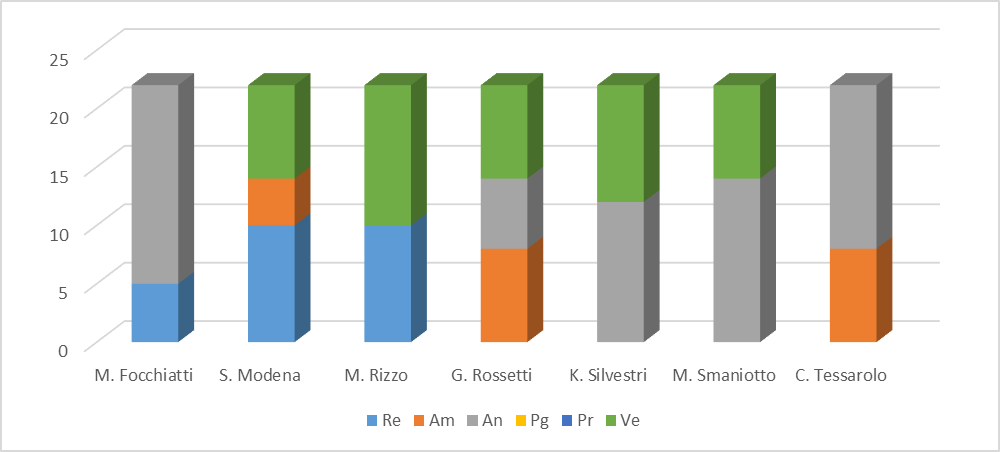
\includegraphics[width=1\linewidth]{img/grafici/AnalisiProspettoOrario}
	\caption{Grafico suddivisione oraria del periodo di Analisi}
	\label{fig:analisi-prospetto-orario}
\end{figure}

\subsection{Prospetto Economico}
Nello svolgimento delle attività di questo periodo i costi sostenuti per ogni ruolo, non a carico del proponente trattandosi dell’investimento iniziale, sono riassunti nella seguente tabella:

\begin{table}[H]
	\centering
	\begin{tabular}{|c|c|c|}
		\hline
		Ruolo&Ore&Costo in \euro{} \\ \hline
		Responsabile&24&720,00  \\ \hline
		Amministratore&20&400,00  \\ \hline
		Analista&61&1525,00  \\ \hline
		Progettista& &  \\ \hline
		Programmatore& &  \\ \hline
		Verificatore&46&690,00  \\ \hline
		Totale&151&3335,00 \\ \hline
	\end{tabular}
	\caption{Prospetto economico del periodo di Analisi}
\end{table}

La ripartizione delle ore tra i vari ruoli è rappresentata graficamente tramite il seguente diagramma a torta:

\begin{figure}[H]
	\centering
	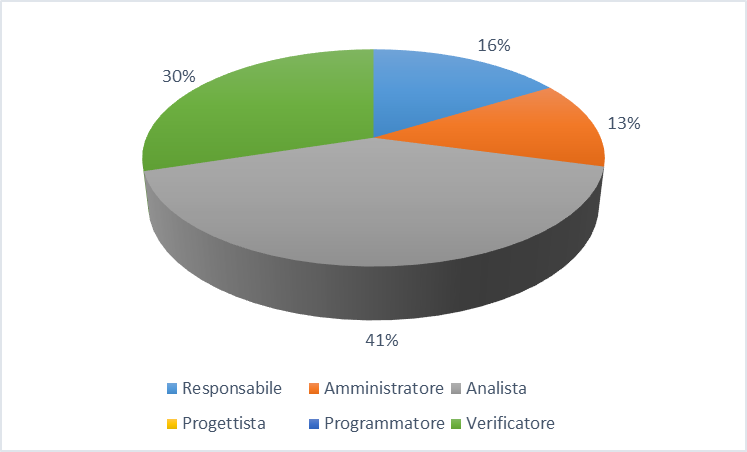
\includegraphics[width=1\linewidth]{img/grafici/AnalisiProspettoEconomico}
	\caption{Grafico suddivisione dei ruoli del periodo di Analisi}
	\label{fig:analisi-prospetto-economico}
\end{figure}


\section{Consolidamento dei requisiti}
Questo periodo di lavoro fa parte del periodo del preventivo.
\subsection{Prospetto Orario}
Nel periodo di Consolidamento dei requisiti la distribuzione oraria sarà la seguente:

\begin{table}[H]
	\centering
	\begin{tabular}{|c|cccccc|c|}
		\hline
		Nominativo&Re&Am&An&Pt&Pr&Ve&Ore totali\\ \hline
		Marco Focchiatti&7&5& &9& &9&30 \\ \hline
		Samuele Modena& & &12&13&5& &30 \\ \hline
		Matteo Rizzo& & &12&14& &4&30 \\ \hline
		Giulio Rossetti& & &5&13& &12&30 \\ \hline
		Kevin Silvestri&8&6& & &7&10&31 \\ \hline
		Manfredi Smaniotto& &7& &18& &5&30 \\ \hline
		Cristiano Tessarolo& & & &23& &7&30 \\  \hline
		Ore totali ruolo&15&18&29&90&12&47&211 \\ \hline
	\end{tabular}
	\caption{Distribuzione oraria del periodo di Consolidamento dei requisiti}
\end{table}

Tali dati sono riassunti graficamente nel seguente diagramma a barre:
\begin{figure}[H]
	\centering
	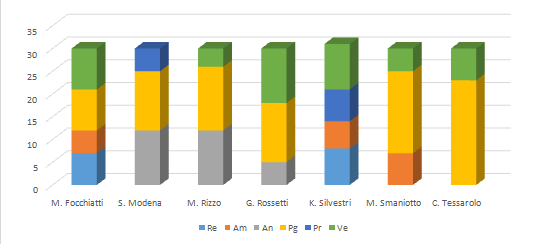
\includegraphics[width=1\linewidth]{img/grafici/ConsolidamentoProspettoOrario}
	\caption{Grafico suddivisione oraria del periodo di Consolidamento dei requisiti}
	\label{fig:consolidamento-prospetto-orario}
\end{figure}

\subsection{Prospetto Economico}
Nello svolgimento delle attività di questo periodo i costi sostenuti per ogni ruolo sono riassunti nella seguente tabella:

\begin{table}[H]
	\centering
	\begin{tabular}{|c|c|c|}
		\hline
		Ruolo&Ore&Costo in \euro{} \\ \hline
		Responsabile&15&450,00  \\ \hline
		Amministratore&18&360,00  \\ \hline
		Analista&29&725,00  \\ \hline
		Progettista&90&1980,00  \\ \hline
		Programmatore&12&180,00  \\ \hline
		Verificatore&47&705,00  \\ \hline
		Totale&211&4400,00 \\ \hline
	\end{tabular}
	\caption{Prospetto economico del periodo di Consolidamento dei requisiti}
\end{table}

La ripartizione delle ore tra i vari ruoli è rappresentata graficamente tramite il seguente diagramma a torta:
\begin{figure}[H]
	\centering
	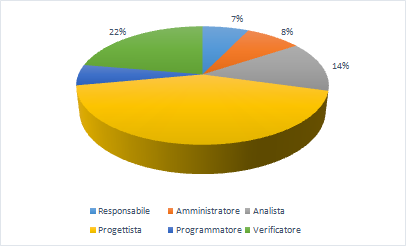
\includegraphics[width=1\linewidth]{img/grafici/ConsolidamentoProspettoEconomico}
	\caption{Grafico suddivisione dei ruoli del periodo di Consolidamento dei requisiti}
	\label{fig:consolidamento-prospetto-economico}
\end{figure}

\section{Progettazione e codifica}
Questo periodo di lavoro fa parte del periodo del preventivo.
\subsection{Prospetto Orario}
Nel periodo di Progettazione di dettaglio e codifica la distribuzione oraria sarà la seguente:

\begin{table}[H]
	\centering
	\begin{tabular}{|c|cccccc|c|}
		\hline
		Nominativo&Re&Am&An&Pt&Pr&Ve&Ore totali\\ \hline
		Marco Focchiatti& & & &30&22& &52 \\ \hline
		Samuele Modena& & & &16&10&26&52 \\ \hline
		Matteo Rizzo& &8& &14&22&8&52 \\ \hline
		Giulio Rossetti& & &&24&22&6&52 \\ \hline
		Kevin Silvestri& & &5&30&17& &52 \\ \hline
		Manfredi Smaniotto&6& & &5&17&24&52 \\ \hline
		Cristiano Tessarolo&8& & & &21&23&52 \\  \hline
		Ore totali ruolo&14&8&5&119&131&87&364 \\ \hline
	\end{tabular}
	\caption{Distribuzione oraria del periodo di Progettazione e codifica}
\end{table}

Tali dati sono riassunti graficamente nel seguente diagramma a barre:
\begin{figure}[H]
	\centering
	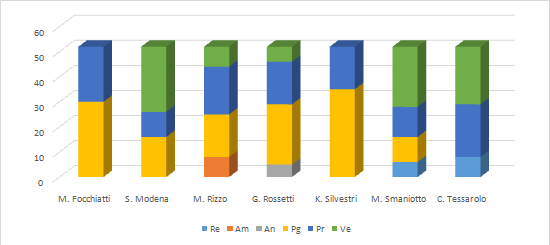
\includegraphics[width=1\linewidth]{img/grafici/ProgettazioneCodificaProspettoOrario}
	\caption{Grafico suddivisione oraria del periodo di Progettazione e codifica}
	\label{fig:progettazione-codifica-prospetto-orario}
\end{figure}

\subsection{Prospetto Economico}
Nello svolgimento delle attività di questo periodo i costi sostenuti per ogni ruolo sono riassunti nella seguente tabella:

\begin{table}[H]
	\centering
	\begin{tabular}{|c|c|c|}
		\hline
		Ruolo&Ore&Costo in \euro{} \\ \hline
		Responsabile&14&420,00  \\ \hline
		Amministratore&8&160,00  \\ \hline
		Analista&5&125,00 \\ \hline
		Progettista&119&2618,00  \\ \hline
		Programmatore&131&1965,00  \\ \hline
		Verificatore&87&1305,00  \\ \hline
		Totale&364&6593,00 \\ \hline
	\end{tabular}
	\caption{Prospetto economico del periodo di Progettazione e codifica}
\end{table}

La ripartizione delle ore tra i vari ruoli è rappresentata graficamente tramite il seguente diagramma a torta:

\begin{figure}[H]
	\centering
	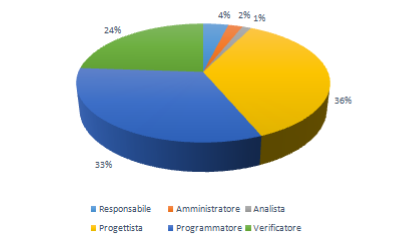
\includegraphics[width=1\linewidth]{img/grafici/ProgettazioneCodificaProspettoEconomico}
	\caption{Grafico suddivisione dei ruoli del periodo di Progettazione di dettaglio e codifica}
	\label{fig:progettazione-codifica-prospetto-economico}
\end{figure}

\section{Validazione e collaudo}
Questo periodo di lavoro fa parte del periodo del preventivo.
\subsection{Prospetto Orario}
Nel periodo di Validazione e collaudo la distribuzione oraria sarà la seguente:

\begin{table}[H]
	\centering
	\begin{tabular}{|c|cccccc|c|}
		\hline
		Nominativo&Re&Am&An&Pt&Pr&Ve&Ore totali\\ \hline
		Marco Focchiatti& & & &2& &18&20 \\ \hline
		Samuele Modena& &6& & &14& &20 \\ \hline
		Matteo Rizzo& &2& &6& &12&20 \\ \hline
		Giulio Rossetti&10& & &6& &4&20 \\ \hline
		Kevin Silvestri& &2& & &5&13&20 \\ \hline
		Manfredi Smaniotto&2&4& &4&4&6&20 \\ \hline
		Cristiano Tessarolo& & & &4& &16&20 \\  \hline
		Ore totali ruolo&12&14& &22&23&69&140 \\ \hline
	\end{tabular}
	\caption{Distribuzione oraria del periodo di Validazione e collaudo}
\end{table}

Tali dati sono riassunti graficamente nel seguente diagramma a barre:
\begin{figure}[H]
	\centering
	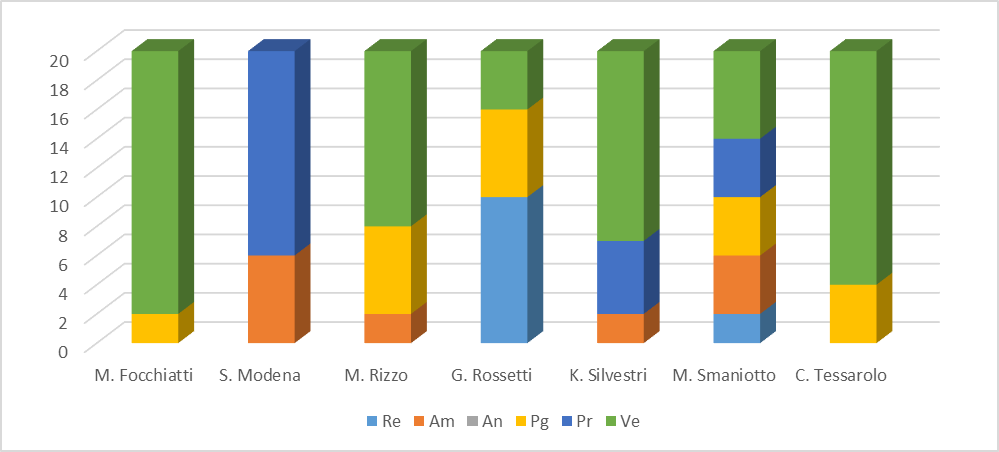
\includegraphics[width=1\linewidth]{img/grafici/ValidazioneCollaudoProspettoOrario}
	\caption{Grafico suddivisione oraria del periodo di Validazione e collaudo}
	\label{fig:validazione-collaudo-prospetto-orario}
\end{figure}

\subsection{Prospetto Economico}
Nello svolgimento delle attività di questo periodo i costi sostenuti per ogni ruolo, non a carico del proponente trattandosi dell’investimento iniziale, sono riassunti nella seguente tabella:

\begin{table}[H]
	\centering
	\begin{tabular}{|c|c|c|}
		\hline
		Ruolo&Ore&Costo in \euro{} \\ \hline
		Responsabile&12&360,00  \\ \hline
		Amministratore&14&280,00  \\ \hline
		Analista& &  \\ \hline
		Progettista&22&484,00  \\ \hline
		Programmatore&23&345,00  \\ \hline
		Verificatore&69&1035,00  \\ \hline
		Totale&140&2504,00 \\ \hline
	\end{tabular}
	\caption{Prospetto economico del periodo di Validazione e collaudo}
\end{table}

La ripartizione delle ore tra i vari ruoli è rappresentata graficamente tramite il seguente diagramma a torta:

\begin{figure}[H]
	\centering
	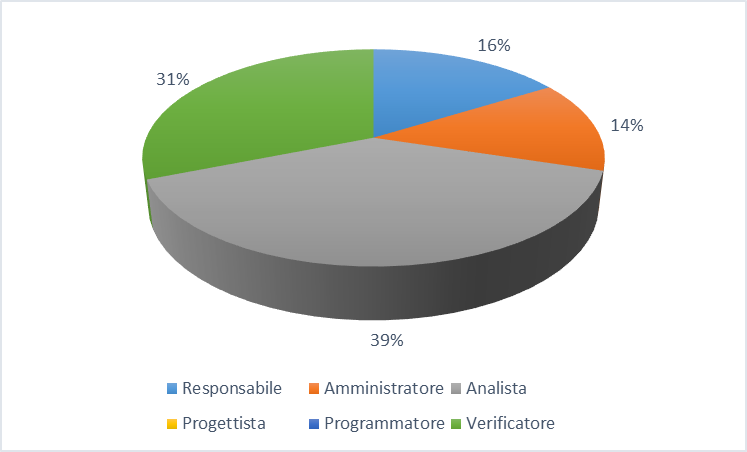
\includegraphics[width=1\linewidth]{img/grafici/ValidazioneCollaudoProspettoEconomico}
	\caption{Grafico suddivisione dei ruoli del periodo di Validazione e collaudo}
	\label{fig:validazione-collaudo-prospetto-economico}
\end{figure}

\section{Totale}
\subsection{Totale suddivisione ore con investimento}
Di seguito sono riportate il totale delle ore del progetto contando le ore di investimento e delle ore rendicontate nel preventivo a carico del committente:

\begin{table}[H]
	\centering
	\begin{tabular}{|c|cccccc|c|}
		\hline
		Nominativo&Re&Am&An&Pt&Pr&Ve&Ore totali\\ \hline
		Marco Focchiatti&12&5&16&41&22&27&123 \\ \hline
		Samuele Modena&10&10&12&29&29&34&124 \\ \hline
		Matteo Rizzo&9&10&12&34&22&36&123 \\ \hline
		Giulio Rossetti&10&8&11&43&22&30&124 \\ \hline
		Kevin Silvestri&8&8&16&30&29&33&124 \\ \hline
		Manfredi Smaniotto&8&11&14&27&21&43&124 \\ \hline
		Cristiano Tessarolo&8&8&14&27&21&46&124 \\  \hline
		Ore totali ruolo&65&60&95&231&166&249&866 \\ \hline
	\end{tabular}
	\caption{Distribuzione oraria totale delle ore di investimento e rendicontate}
\end{table}

Tali dati sono riassunti graficamente nel seguente diagramma a barre:
\begin{figure}[H]
	\centering
	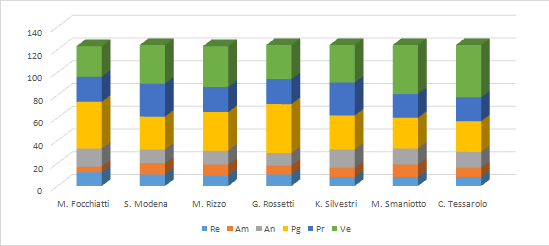
\includegraphics[width=1\linewidth]{img/grafici/OreInvestimentoRendicontateProspettoOrario}
	\caption{Grafico suddivisione oraria totale delle ore di investimento e rendicontate}
	\label{fig:ore-investimento-rendicontate-prospetto-orario}
\end{figure}

\subsection{Totale del prospetto economico con investimento}
Di seguito è riportato il totale delle ore dei diversi ruoli del progetto contando anche le ore di investimento, non a carico del proponente trattandosi dell'investimento iniziale:

\begin{table}[H]
	\centering
	\begin{tabular}{|c|c|c|}
		\hline
		Ruolo&Ore&Costo in \euro{} \\ \hline
		Responsabile&65&1950,00  \\ \hline
		Amministratore&60&1200,00  \\ \hline
		Analista&95&2375,00 \\ \hline
		Progettista&231&5082,00 \\ \hline
		Programmatore&166&2490,00 \\ \hline
		Verificatore&249&3735,00  \\ \hline
		Totale&866&16832,00 \\ \hline
	\end{tabular}
	\caption{Prospetto economico totale delle ore di investimento e rendicontate}
\end{table}

La ripartizione delle ore tra i vari ruoli è rappresentata graficamente tramite il seguente diagramma a torta:

\begin{figure}[H]
	\centering
	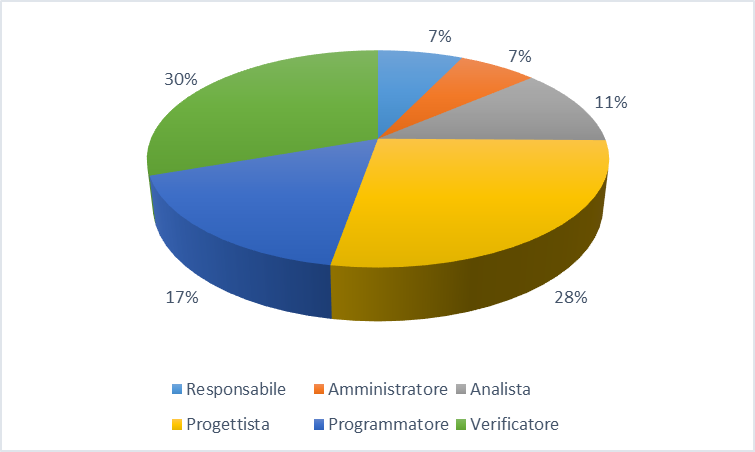
\includegraphics[width=1\linewidth]{img/grafici/OreInvestimentoRendicontateProspettoEconomico}
	\caption{Grafico suddivisione dei ruoli totale delle ore di investimento e rendicontate}
	\label{fig:ore-investimento-rendicontate-prospetto-economico}
\end{figure}


\subsection{Totale suddivisione ore rendicontate}
Di seguito sono riportate il totale delle sole ore rendicontate nel preventivo a carico del committente:

\begin{table}[H]
	\centering
	\begin{tabular}{|c|cccccc|c|}
		\hline
		Nominativo&Re&Am&An&Pt&Pr&Ve&Ore totali\\ \hline
		Marco Focchiatti&7&5& &41&22&27&102 \\ \hline
		Samuele Modena& &6&12&29&29&26&102 \\ \hline
		Matteo Rizzo& &10&12&34&22&24&102 \\ \hline
		Giulio Rossetti&10& &5&43&22&22&102 \\ \hline
		Kevin Silvestri&8&8&5&30&29&23&103 \\ \hline
		Manfredi Smaniotto&8&11& &27&21&35&102 \\ \hline
		Cristiano Tessarolo&8& & &27&21&46&102 \\  \hline
		Ore totali ruolo&41&40&34&231&166&203&715 \\ \hline
	\end{tabular}
	\caption{Distribuzione oraria totale delle ore rendicontate}
\end{table}

Tali dati sono riassunti graficamente nel seguente diagramma a barre:
\begin{figure}[H]
	\centering
	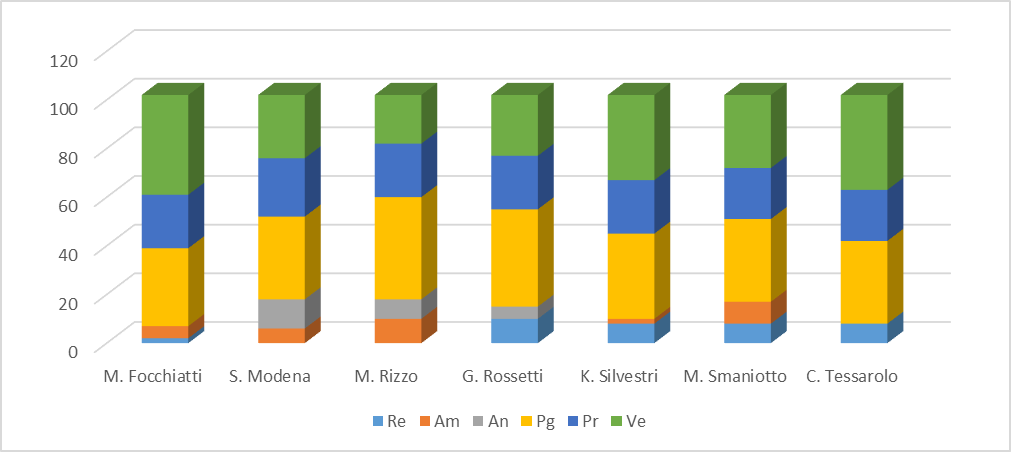
\includegraphics[width=1\linewidth]{img/grafici/OreRendicontateProspettoOrario}
	\caption{Grafico suddivisione oraria totale delle ore rendicontate}
	\label{fig:ore-rendicontate-prospetto-orario}
\end{figure}

\subsection{Totale del prospetto economico rendicontato}
Di seguito è riportato il totale delle ore dei diversi ruoli del progetto contando solo le ore rendicontate nel preventivo a carico del committente cioè dei periodi di Progettazione architetturale, Progettazione di dettaglio e codifica ed il periodo di Validazione e collaudo:

\begin{table}[H]
	\centering
	\begin{tabular}{|c|c|c|}
		\hline
		Ruolo&Ore&Costo in \euro{} \\ \hline
		Responsabile&41&1230,00 \\ \hline
		Amministratore&40&800,00 \\ \hline
		Analista&34&850,00 \\ \hline
		Progettista&231&5082,00 \\ \hline
		Programmatore&166&2490,00 \\ \hline
		Verificatore&203&3045,00 \\ \hline
		Totale&715&13497,00 \\ \hline
	\end{tabular}
	\caption{Prospetto economico totale delle ore rendicontate}
\end{table}

La ripartizione delle ore tra i vari ruoli è rappresentata graficamente tramite il seguente diagramma a torta:

\begin{figure}[H]
	\centering
	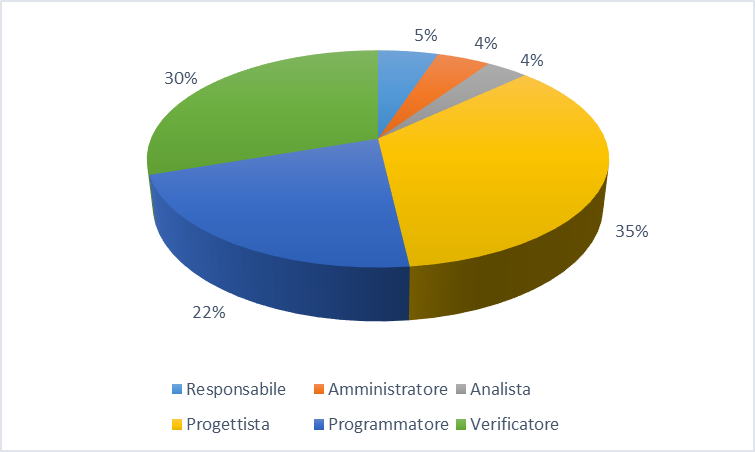
\includegraphics[width=1\linewidth]{img/grafici/OreRendicontateProspettoEconomico}
	\caption{Grafico suddivisione dei ruoli totale delle ore rendicontate}
	\label{fig:ore-rendicontate-prospetto-economico}
\end{figure}

\section{Conclusione}
Il costo totale preventivato per il progetto è di 13497,00 \euro{}.

\end{document}